
\section{Lecture 10: Hooke's law, simple harmonic oscillator}

Say we have a spring, in its ``relaxed'' state, i.e. in equilibrium. We choose to place $x = 0$ at the spring's end, and then extend the spring a distance $x$.

There will be a restoring force that attempts to pull the spring back to its original length. For many springs, it is approximately true that this restoring force $F$ is proportional to the displacement $x$.\\
For an \emph{ideal spring}, we can write the force as

\begin{equation}
F = -k x
\end{equation}

where $k$ is known as the spring constant, and the minus sign signifies that the force opposes the displacement. (If $x$ is positive to the right, the force will be to the left, and vice versa.)\\
This also holds if the spring is compressed (shortened) instead of stretched.\\
The above relation is known as \emph{Hooke's law}.

We can measure this spring constant in a few different ways. Perhaps the simplest would be to hang a mass from a spring and measure how far it extends due to the pull of gravity. When it is in equilibrium, we know that the upwards force from the spring must equal the downwards force due to gravity. Therefore, we can measure $x$ and $m$, and we know $g$, so we can calculate the spring constant:

\begin{align}
|F| = k x &= m g\\
k &= \frac{m g}{x}
\end{align}

Assuming we work in SI units, the units of the spring constant must then be in newtons per meter.

If we instead change the masses, we will get a plot that is a straight line, assuming Hooke's law holds. We can then find $k$ as the slope of this line:

\begin{center}
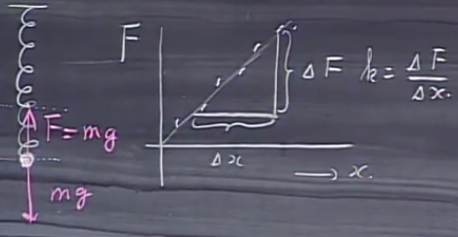
\includegraphics[scale=0.7]{\pIImages/lec10_measure}
\end{center}

This is probably a more reliable test than the single calculation above, since it will show if Hooke's law doesn't hold for the particular spring, instead of silently assuming that it does.

Hooke's law has its limitations, as you might expect. It's possible to stretch a spring so far that it permanently changes its shape, in which case the restoring force will not increase linearly, but grow slower than Hooke's law would predict.

Let's look at a second way of measuring the spring constant of a given spring. Say we have another spring, again with $x = 0$ at the end of spring's relaxed length. We extend the spring further, and attach a mass $m$ to the end of the spring. The mass rests on a frictionless surface.

\begin{center}
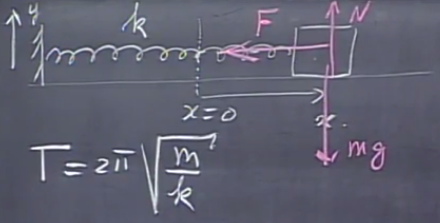
\includegraphics[scale=0.7]{\pIImages/lec10_sho}
\end{center}

When we let the mass go, this system will begin to oscillate. The spring force pulls the mass towards the left until it is relaxed, but when that happens, the mass is already moving towards the left, and has inertia in that direction. The spring will be compressed, and now push on the mass, which eventually comes to a halt, accelerates back towards the right, etc.

Because of the relationship shown, which will be derived shortly, we can either calculate a spring constant from a known mass (while using a stopwatch), or me can measure a mass, if we know the spring constant, even in the absence of gravity! Note that there is no relation to $g$ in the formula. The only place where it appears is in the pull of gravity and the normal force, but since the surface is taken to be frictionless, neither force matters for the oscillation period.

It's interesting to note that the amplitude of the oscillation, i.e. how far it moves horizontally from the center point, does not affect the period at all. If the amplitude is small, it will move slowly back and forth, but if the amplitude is large, it will move at much greater speed, to keep the period constant -- assuming Hooke's Law holds.

\subsection{Simple harmonic oscillators: mathematical derivation}

Let's have a look at the situation we have above. We apply Newton's second law to the system, and find

\begin{equation}
m a = - k x
\end{equation}

Written in alternative notation, and divided through by $m$:

\begin{align}
m \ddot{x} + k x = 0\\
\ddot{x} + \frac{k}{m} x = 0
\end{align}

$\dot{x}$ is used to signify the first time derivative of position (velocity), while $\ddot{x}$ is used for the second time derivative (acceleration).

Prof. Lewin calls this last equation ``arguably the most important in all of physics''. It is the equation that governs simple harmonic oscillators; there are many kinds of such oscillators.

First, it is demonstrated that the solution for $x(t)$ should be some form of sinusoid. Trying to keep this as general as possible, we can write

\begin{equation}
x = A \cos(\omega t + \varphi)
\end{equation}

Here, $A$ is the amplitude (how far it swings, from the center point), $\omega$ is the \emph{angular frequency} (not to be confused with angular velocity), in radians/second, and $\varphi$ is the \emph{phase angle}, in radians.

As we have seen many times before,

\begin{equation}
T = \frac{2 \pi}{\omega}
\end{equation}

since if you increase $t$ by $T$ seconds, the argument to the cosine will have increased by $2 \pi$ radians $= \ang{360}$, and the function repeats.

We can write this in terms of frequency (``regular'' frequency in Hertz, i.e. the number times something happens per second, rather than angular frequency):

\begin{equation}
f = \frac{1}{T} = \frac{\omega}{2 \pi}
\end{equation}

(We can think of the last equations as being in radians per second, divided by $2 \pi$ radians; the ``per second'' is then all that remains.)

Next, we substitute our ``trial answer'' into the equation relating $x$ and $\ddot{x}$. To do that, we must first find $\ddot{x}$, i.e. the second derivative of $x$ with respect to time. Keeping in mind the chain rule, we find

\begin{align}
x        &= A \cos(\omega t + \varphi)\\
\dot{x}  &= A \omega (-\sin(\omega t + \varphi) = -A \omega \sin(\omega t + \varphi)\\
\ddot{x} &= -A \omega^2 \cos(\omega t + \varphi)
\end{align}

Now, because $x = A \cos(\omega t + \varphi)$, we can also write

\begin{align}
\ddot{x} = -\omega^2 x
\end{align}

All in all, our differential equation becomes

\begin{equation}
- \omega^2 x + \frac{k}{m} x = 0
\end{equation}

Because this must always hold for all $x$, it must be the case that

\begin{align}
w^2 = \frac{k}{m}\\
\omega = \sqrt{\frac{k}{m}}
\end{align}

With the equation we already had for $T$, it turns out that

\begin{align}
T = 2 \pi \sqrt{\frac{m}{k}}
\end{align}

... as shown in the figure prior to this derivation.

As we can see, the period is independent on the amplitude, and also independent on the phase angle $\varphi$. More on that now.

When we start this oscillation, we can decide two things: how far we stretch the spring before we let the mass go, and how much (if any) of a push we give it, i.e. initial velocity. The amplitude and phase angle will be decided by these \emph{initial conditions}.

Say we give it a push, so that $\vec{v} = -3\hat{x}$ m/s, while it is at $x = 0$ at $t = 0$. With all these conditions, we can find both the amplitude $A$ and the phase angle $\varphi$. We know the equation must hold true at $x = 0$ at $t = 0$, since that's a given, so we plug that in:

\begin{align}
0 = A \cos(\varphi)
\end{align}

This equation can be true in two cases: $A = 0$, or $\cos(\varphi) = 0$. $A$ cannot be 0, because we know there will be an oscillation with a nonzero amplitude. Therefore,

\begin{align}
\cos(\varphi) = 0\\
\varphi = \frac{\pi}{2}, \frac{3\pi}{2}
\end{align}

Either value of $\varphi$ makes the cosine zero. (There are of course an infinite number of such angles, but we restrict them to $0 < \varphi < 2\pi$.)

Since we have a time-varying position, we can take the time derivative to find the velocity as a function of time, and relate that to the initial condition $v = -3$ m/s.

We calculate the time derivative of the equation (which we did earlier), and substitute in the values, including $t = 0$, and set it equal to $-3$ m/s:

\begin{align}
x = A \cos(\omega t + \varphi)\\
\dot{x} = -A \omega \sin(\omega t + \varphi)
\end{align}

Keep in mind that $\dot{x} = v$.\\
In with the values, and solve:

\begin{align}
-3 = -A \omega \sin(\pi/2)\\
-A \omega = -3\\
A = \frac{3}{\omega}
\end{align}

Say the object has a mass $m = \SI{0.1}{kg}$, and the spring has a spring constant of $k = \SI{10}{N/m}$.

We find $\omega$ as

\begin{equation}
\omega = \sqrt{\frac{k}{m}} = 10 \text{ rad/s}
\end{equation}

So $A = 0.3$ meters, and the full equation that explains this oscillation is

\begin{equation}
x(t) = 0.3 \cos(10 t - \frac{\pi}{2})
\end{equation}

\subsection{Motion of a pendulum}

Next up, we have a look at the equations that govern a pendulum's motion.

\begin{center}
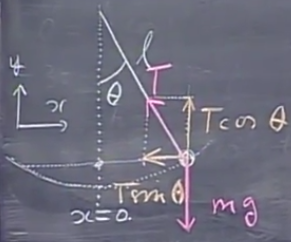
\includegraphics[scale=0.7]{\pIImages/lec10_pendulum}
\end{center}

We have a mass $m$ attached to a string of length $\ell$, which is swinging back and forth. We choose a coordinate system with its origin at the pendulum's center, decompose the forces, and write down Newton's second law for the system.

Gravity is pulling downwards on the mass, while there is a tension in the string pulling upwards (but not straight upwards, of course). We decompose this tension, and write down the equation for the $x$ direction:

\begin{equation}
m a_x = m\ddot{x} = - T(\theta) \sin \theta = -T(\theta) \frac{x}{\ell}
\end{equation}

$a$ is towards the right (since that is the positive direction of the coordinate system), but the horizontal component of the tension is towards the left at this moment. The second equality holds for trigonometric reasons.

For the $y$ direction, we find

\begin{equation}
m \ddot{y} = T(\theta) \cos \theta - m g
\end{equation}

We then have two coupled differential equations to solve, which is above this course's level... but we can simplify things a bit.\\
We start out by making some approximations. First out is the small angle approximation, which is usually used to imply that $\sin \theta \approx \theta$ and $\cos \theta \approx 1$ if $\theta \ll 1$ radian (it works quite well up to 0.2 rad $\approx \ang{11.5}$ or so, at least, where $\cos(0.2) \approx 0.98$ and $\sin(0.2) \approx 0.1987$).

There is a second important approximation we can make if we assume the angle will always be small. Have a look at the diagram above, and note how the $x$ amplitude is much greater than the $y$ amplitude. For a 5 degree swing, the $x$ motion is about 25 times as large as the $y$ motion, and it is still 11 times as large at 10 degrees.\\
We can therefore approximate the acceleration in the $y$ direction to be zero, so we find

\begin{align}
0 = T(\theta) - m g\\
T = m g
\end{align}

The cosine disappears, since we approximated it to be one, and the left-hand side disappears since $a = \ddot{x} \approx 0$.

We substitute this into our differential equation for $x$, and find

\begin{align}
m\ddot{x} = -m g \frac{x}{\ell}\\
m\ddot{x} + m g \frac{x}{\ell} = 0\\
\ddot{x} + \frac{g}{\ell} x = 0
\end{align}

Compare this to the spring-mass system, which obeyed $\displaystyle \ddot{x} + \frac{k}{m} x = 0$ -- this is another simple harmonic oscillator!

Since the only difference between the differential equations is, practically, two variable names, the solution is of course the same. We find these equations for this system:

\begin{align}
x = A \cos(\omega t + \varphi)\\
\omega = \sqrt{\frac{g}{\ell}}\\
T = \frac{2 \pi}{\omega} = 2 \pi \sqrt{\frac{\ell}{g}}
\end{align}

Keep in mind that these results are limited to the case where the angles are small, and the string can be considered massless in comparison to the mass at the end of the string.

Now, let's compare the results we found for the spring/mass system and the pendulum on a string.\\
For the oscillating spring, the period depends on the spring constant and the mass $m$. This can be explained simply, as follows: when you extend a spring, there is a restoring force, proportional to the distance you extended it. However, the force is not in any way dependent on the mass of the object you attach to the spring; therefore, the acceleration is inversely proportional to the mass, via Newton's second law:

\begin{align}
|a| = \frac{|F_{spring}|}{m} = \frac{k |x|}{m}
\end{align}

If the acceleration is very low, clearly the period must increase.

As for the pendulum, the period is independent on the mass. Why?\\
Again, this can be shown quite easily. If $m$ doubles, $m g$ doubles, and so the tension $T = m g$ must also double (since the $y$ acceleration is the same -- approximately zero). The restoring force $T \sin \theta$ is proportional to $T$, so that doubles as well. If the mass doubles and the force doubles, the acceleration stays exactly the same, and so the period is not affected.

Next, $k$ and $g$. If $k$ is high, the period is short, which makes sense: the acceleration is proportional to $\sqrt{k}$, so for very large $k$ (meaning a very stiff/strong spring -- remember that it's in newtons per meter of displacement) the acceleration is high, and the period low.\\
As for the pendulum, it is \emph{inversely} proportional to $\sqrt{g}$, so if $g$ is low, the period is very large, and it goes to infinity as $g \to 0$. A pendulum could not work in weightlessness, where the perceived gravity is zero, since it relies on gravity to swing. (This too is easy to see: the restoring force is proportional to $g$, so with $g \approx 0$, there shouldn't be any restoring force, nor any string tension.)

``All'' that remains in the lecture is one of the best demonstrations in this class, which means no notes taken, but careful watching instead!

\section{Lecture 11: Work, energy and universal gravitation}

Let's get started right away.\\
\emph{Work} is a measure of the amount of energy a force uses when moving an object. In simple applications, it can be defined as $W = F d$, where $F$ is the magnitude of the force, and $d$ is the distance the object moves.

A more useful definition, still in one dimension, is an integral, which then can take care of non-constant forces as well:

\begin{equation}
W_{AB} = \int_A^B F\ \mathop{dx}
\end{equation}

... where $A$ and $B$ are the $x$ coordinates where the object starts out, and ends up, respectively.

Work is a scalar quantity, and can be negative, zero or positive.\\
It is positive if the force and the displacement are in the \emph{same} direction, and negative if they are in the \emph{opposite} direction. It can be zero, e.g. if there is no displacement.

The SI unit of work is the joule, J, which from the definition clearly is the same as a force of 1 newton times a displacement of 1 meter. We rarely if ever write Nm for work; though Nm and J are mathematically equivalent, Nm is used for torque (which will be introduced later in the course).

Since $\displaystyle F = m a = m \frac{dv}{dt}$, and distance $dx = v dt$, we can rewrite this integral in terms of velocity:

\begin{equation}
W_{AB} = \int_A^B m \frac{dv}{dt} v \mathop{dt} = \int_{v_A}^{v_B} m\ v \mathop{dv} = \Big[ \frac{1}{2} m v^2 \Big]_{v_A}^{v_B} = \frac{1}{2} m \left(v_B^2 - v_A^2\right)
\end{equation}

Here, we have also found the formula for kinetic energy, often notated as $K_E$, $K_e$ or just $K$:

\begin{equation}
K_E = \frac{1}{2} m v^2
\end{equation}

If an object of mass $m$ is moving at velocity $v$, the above formula can calculate its kinetic energy, i.e. how much energy is required to accelerate it to that velocity.

In other words, using the above two relations, we can see that

\begin{equation}
W_{AB} = \Delta K_E = K_{EB} - K_{EA}
\end{equation}

This is known as the \emph{work-energy theorem}. The difference in kinetic energy of an object is equal to the amount of work done on it by the net forces acting on it.\\
If the kinetic energy has increased when moving from point A to point B, the work is positive; if the kinetic energy has decreased, the work is negative, and if the kinetic energy is unchanged, the net work is zero.\\
Note that it's positive for multiple forces to work against each other, such that one provides positive work, a different force provides negative work, etc. such that the \emph{net} work, and thus the change in kinetic energy, can be either positive, negative or zero, depending on the strengths and angles of the forces.

Let's try an applied example. Say an object is moving upwards, while gravity acts on it downwards as you'd expect.\\
We choose the positive $y$ axis to be upwards, so gravity is $-mg\hat{y}$. The object has a velocity $v_A$ where it starts out at point A, and moves upwards to point B while losing speed due to gravity.

We now want to calculate the distance $h$ between points A and B, assuming that the object comes to (temporary) rest at point B.\\
We apply the work-energy theorem, with $\displaystyle K_{EA} = \frac{1}{2} m v_A^2$ and $K_{EB} = 0$.\\
The gravitational force is constant with a magnitude of $m g$, so the work gravity does is $m g h$. The direction of the force is downward, and the motion is upwards, so the work is negative.\\
We set the two equal and solve for $h$:

\begin{align}
- m g h = 0 - \frac{1}{2} m v_A^2\\
g h = \frac{1}{2} v_A^2\\
h = \frac{v_A^2}{2 g}
\end{align}

We have seen this result before, but we found it in a quite different way last time.

As a second example, say we lift an object against gravity, a height $h$ above where it started out. It starts with 0 speed, and also ends up with 0 speed. Via the work-energy theorem, the net work must be zero, since the object's kinetic energy did not change.\\
Gravity still does its work of $|F h| = |m g h|$, only that it's negative here: the force direction is down, and the motion is up. Since gravity does work $- m g h$ on the object, we, who lift it, must then provide positive work $m g h$ in order to make the net work zero.

If we instead reverse the situation, and lower the object closer to the ground, the opposite thing happens. Gravity does positive work $m g h$, while we provide negative work $- m g h$ when lowering the object, and again the net work must be zero, if the object both starts out and ends up with no kinetic energy.

It's important to realize that work, as used in physics, is far from the same as we might think intuitively.\\
If we lower a very heavy object from a height down to the ground, we will have provided negative work, $- m g h$, but we for sure have still \emph{spent} energy burned in our muscles to provide it. We didn't get some sort of added energy reserve from doing so, even though the work is negative.\\
Likewise, we can get tired from holding an object perfectly still (try holding something heavy at arm's length for an extended period of time!), despite the fact that $F d = 0$ and no work has been done.

\subsection{Taking the step to three dimensions}

We can extend what we have above to three dimensions. Say we apply a force $\vec{F}$ over a path. For each tiny point of this path, we can find a vector $\vec{dr}$, which represents a infinitesimal displacement along the line; so small that we can approximate it as a straight line, rather than some form of curve.

\begin{center}
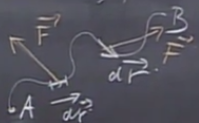
\includegraphics[scale=0.8]{\pIImages/lec11_work_3d}
\end{center}

The net work done by the force over the entire path is

\begin{equation}
W_{AB} = \int_A^B = \vec{F} \cdot \vec{dr}
\end{equation}

A dot product integral may look scary, but they're not too bad.\\
By the way, the above is a \emph{line integral} (or \emph{path integral}, or \emph{contour integral}): it evaluates an integral along a path.

We can decompose this integral into three one-dimensional integral -- surprise! -- to make it easier to solve. In general terms, we can write the force vector and the displacement vector as sums of components:

\begin{align}
\vec{F}  &= F_x \hat{x} + F_y \vec{y} + F_z \hat{z}\\
\vec{dr} &= dx \hat{x} + dy \hat{y} + dz \hat{z}
\end{align}

With this in mind, we can find $dW$, a small amount of work done by the force over a small distance $dr$, using the definition of the dot product:

\begin{equation}
dW = \vec{F} \cdot \vec{dr} = F_x \mathop{dx} + F_y \mathop{dy} + F_z \mathop{dz}
\end{equation}

Integrate both sides, and we find

\begin{align}
W_{AB} = \int_A^B \vec{F} \cdot \vec{dr} &= \int_A^B \left(F_x \mathop{dx} + F_y \mathop{dy} + F_z \mathop{dz}\right)\\
                                    &= \int_A^B F_x \mathop{dx} + \int_A^B F_y \mathop{dy} + \int_A^B F_z \mathop{dz}
\end{align}

We now have three one-dimensional problems to solve, instead. Not only that, but we've already solved this integral in one dimension. We just need to add it up for the three dimensions:

\begin{equation}
W_AB = \frac{1}{2} m \left( v_{Bx}^2 - v_{Ax}^2 \right) + \frac{1}{2} m \left( v_{By}^2 - v_{Ay}^2 \right) + \frac{1}{2} m \left( v_{Bz}^2 - v_{Az}^2 \right)
\end{equation}

Not pretty... but that's probably the last time we'll see it written like that. Here it is again, re-arranged, but exactly equal to the above:

\begin{align}
W_AB &= \frac{1}{2} m \left( v_{Bx}^2 + v_{By}^2 + v_{Bz}^2 \right) - \frac{1}{2}m  \left( v_{Ax}^2 + v_{Ay}^2 + v_{Az}^2 \right)\\
     &= \frac{1}{2} m \left( v_B^2 - v_A^2 \right)
\end{align}

... and so we find exactly the same result as we did in one dimension.

Let's as an example calculate the work done by gravity while moving an object around in 3D space.

\begin{center}
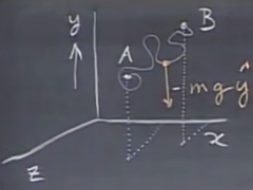
\includegraphics[scale=0.8]{\pIImages/lec11_3d_path}
\end{center}

We move from a point $A$ to a point $B$, where $y_B - y_A = h > 0$, in other words, point B is higher up than point A.

The force due to gravity is $- m g \hat{y}$, so the integral would be

\begin{equation}
W_{gravity} = \int_A^B \vec{F} \cdot \vec{dr} = \int_A^B (- m g) \mathop{dy} = - m g \int_A^B \mathop{dy} = -m g(y_B - y_A) = -m g h
\end{equation}

The $x$ and $z$ terms disappear, since $F_x = 0$ and $F_z = 0$ -- gravity only acts along one axis, with the way we've defined our coordinate system.

We find that the work done by gravity is negative, as it should be -- the force vector is down, but the object moved higher up. The net work of the force(s) that moved it upwards, in the $y$ direction, is then $+ m g h$.\\
(We can't say anything about the work along the $x$ and $z$ axes without more information, of course.)

Another thing is interesting about this result: it is independent of the path between points A and B. The only thing that matters, as far as gravity is concerned, is the difference in height. If you move an object up 10 meters and back down 9, the work done by gravity is exactly the same as if you'd just moved it up the one meter. The same goes for all and any movement in the x-z plane, which doesn't affect the work done by gravity whatsoever.

Any force that has the property that the work done is the same for any given pair of start/end points, regardless of the path moved in between them, is called a \emph{conservative force}. As we have just shown, gravity is conservative. If a particle starts at one point, moves around in any path whatsoever, and comes back to that exact point, the work done by gravity is always zero.

\subsection{Conservation of mechanical energy}

We can apply the work-energy theorem to the equation above:

\begin{align}
-m g(y_B - y_A)& = K_{EB} - K_{EA}\\
-m g\ y_B - m g\ y_A &= K_{EB} - K_{EA}\\
K_{EA} + m g\ y_A &= K_{EB} + m g\ y_B
\end{align}

This is a very important result. The quantity $m g y$ is what we call \emph{gravitational potential energy}, often $P_E$ or $U$. What the above result says, then, is that the sum of the kinetic and potential energies at point A must equal the sum of the kinetic and potential energies at point B.

\begin{equation}
K_{EA} + U_A = K_{EB} + U_B
\end{equation}

This is known as the \emph{conservation of mechanical energy}, where the mechanical energy of an object is the sum of its kinetic energy and its potential energy. One can be converted into the other, but \emph{as long as the forces involved are conservative}, the sum of the two must stay equal. This condition is an important one! Friction, for example, is \emph{not} a conservative force, and this relationship will no longer hold if frictional forces are involved.\\
Spring forces \emph{are} conservative, however.

The fact that frictional forces are not conservative should be fairly intuitive. The further we move something against friction, the more total work must be done to overcome the friction. You could move something back and forth on a table and the work done by the friction (and you, in moving it) would just increase and increase in magnitude.\\
If you did the same against gravity, moving something up, then back down, etc., the work done (by gravity, or by you) would \emph{not} simply increase without bound.

With the definition of $K_E = \frac{1}{2} m v^2$, it's clear that kinetic energy is zero when the velocity $v$ of an object is zero.\\
What about potential energy? That is zero where $y = 0$, but where is that? It is up to us to decide where to place that point. We are free to choose it, as long as $g$ is the same at both point $A$ and point $B$ (or simply that $g$ is close enough, so that we can neglect the difference).

\subsubsection{Example problem}

\begin{center}
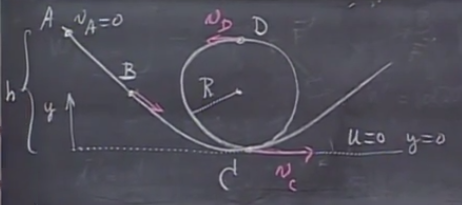
\includegraphics[scale=0.8]{\pIImages/lec11_conservation}
\end{center}

We place an object on this ``roller coaster'', at point A, which is $h$ above the line where we choose $y = 0$ and $U = 0$. It gains speed, by converting gravitational potential energy to kinetic energy, until it reaches point C, where the velocity (and the kinetic energy) is at a maximum, while the potential energy is zero, by our definition.

At that point, it reaches the loop. The question is: from what height $h$ must we let it go along the track, so that it manages to move around the loop without falling out before reaching the top?

We can apply the conservation of mechanical energy to this problem, assuming friction is negligible:

\begin{equation}
U_A + K_{EA} = U_B + K_{EB} = U_C + K_{EC} = U_D + K_{ED}
\end{equation}

We let it go from rest at point A, so $K_{EA} = 0$. Our definition of potential energy as $U = m g h$, where $h$ is the height above the plane where $U = 0$.\\
The vertical distance is must travel ``upward'' in going around the circle is twice the radius, so $2R$.

If we equate the total mechanical energy at A, $U_A = m g h$, with the total mechanical energy at any given point, we can find

\begin{align}
m g h &= m g y + \frac{1}{2} m v^2\\
v^2   &= 2g (h - y)
\end{align}

This equation should hold for any point, again assuming we can neglect friction and other forces. At point D, at the top of the loop, the constraint that $a_c > g$ must hold, or we know that it will fall out of the loop, instead of being pushed against it by the centripetal force.

Since centripetal acceleration is given by $\displaystyle a_c = \frac{v^2}{r}$, and we know $v^2$, we can write an inequality for this being larger than $g$, and then solve for $h$, to find the answer to our question about the minimum height we must release the object from.\\
$y = 2 R$ at this point, so

\begin{align}
\frac{2g (h - 2R)}{R} &\ge g\\
2 h - 4R &\ge R\\
2 h &\ge 5R\\
h &\ge \frac{5}{2} R
\end{align}

So if we find a point along the roller coaster where this condition is met, and perhaps add a small amount due to friction, the ball will ``make the loop'', so to speak. Without friction, air resistance etc., it would come up to the exact same height as it started rolling down from.

\subsection{Newton's law of universal gravitation}

Like the previous laws we've learned with Newton's name attached to them, the law of universal gravitational is quite simple.

Say we have two masses, often named $m$ and $M$ (where it's often the case that $M$ e.g. a planet, and $m$ is smaller; this is of course no requirement, however). The two point masses\footnote{This also works for masses of nonzero size in some cases, more on that at a later time.} are separated by a distance $r$. The force that $m$ experiences because of $M$ is then

\begin{equation}
F = \frac{G M m}{r^2}
\end{equation}

in the direction of $M$ (gravity is always an attractive force), where $G$ is the gravitational constant, not to be confused with $\displaystyle g \approx \frac{G M_{Earth}}{R_{Earth}^2}$ (approximately because Earth's mass is not all at the center; Earth is not a perfect sphere, etc.).\\
$G$ has a value of about $6.67 \cdot 10^{-11}$, with units that need to cancel out with the others, i.e.

\begin{align}
\text{[N]} = \frac{\text{[G]} \text{[kg]}^2}{\text{[meter]}^2}\\
\frac{\text{[N]} \text{[meter]}^2}{\text{[kg]}^2} = \text{[G]}
\end{align}

So in more terse notation, the units of $G$ are $\text{N} \cdot \text{m}^2 \text{kg}^{-2}$.

Because of $F = ma$, so $\displaystyle a = \frac{F}{m}$, we can find the gravitational acceleration due to a mass $M$ to be the force, above, divided by the mass $m$, as already shown in the aside about $g$.

As the formula shows, as the distance from the source of the gravity doubles, the magnitude of the force (or the acceleration) is reduced by a factor of 4.

\subsection{Gravitational potential energy}

Let's now talk about gravitational potential in the general case. Previously, we've only used it where we are near the surface of the Earth, and $g$ has a value that can be considered constant. This is of course not true in general, but there is a definition we can use that is valid everywhere in the universe.

If it is to be valid everywhere, where do we place the zero? There are only two plausible choices, and one (at $r = 0$) turns out to not make much sense. We end up with only one possibility, which is that $U = 0$ is at $r \to \infty$. This has the strange consequence of making all potential energy values negative, but that does not matter: it is still the \emph{difference} in potential energy that matters, and we could have found negative values with the previous method too, for some choices of the point where $U = 0$.

A general definition of the gravitational potential energy is that $U$ is the amount of work \emph{you} must do to move a mass from infinity to some point P, located some distance from a mass $M$. Alternatively, but equivalently, it's the work gravity does in moving the same mass \emph{from} some point P \emph{to} infinity.

In either case, it's clear that the value must be negative: if the mass is attracted to the point, you don't have to do \emph{any} positive work to move it there, but rather negative work.\\
In the second formulation, gravity doesn't do \emph{any} positive work when you move the mass \emph{away} from another mass, so again the value is negative.

Let's now calculate a general formula for gravitational potential energy. Using the definition above, where it equals the work we do in moving a mass from infinity to P (located $R$ away from the mass $M$),

\begin{align}
U = \int_\infty^R \frac{G M m}{r^2} dr = G M m \int_\infty^R r^{-2} dr = \Big[-\frac{G M m}{r}\Big]_\infty^R = -\frac{G M m}{R}
\end{align}

Note how the value will always be zero ``at'' infinity, and grow larger (\emph{less negative}, but still larger!) as we move away from a body.

\subsubsection{Example calculation}

Lecture question: A mass $M$ is released at zero speed, $2 \cdot 10^6$ km from the center of the Earth. At what speed does it hit the Earth, ignoring the gravitational forces from all other objects in the solar system?

We could integrate the acceleration to find the answer, but that is dependent on time, so that seems more trouble than it's worth.

Let's instead attempt to do this by conservation of energy -- I'm fairly sure that was the intention, anyway.\\
If we assume mechanical energy will be conserved, which ought to be a fairly good approximation here, 100\% of the change in the potential energy is converted to kinetic energy. What is the change in potential energy, $\Delta U$? Using the formula for potential energy above, and using A for the initial location and B at the surface at the Earth, it must be

\begin{align}
\Delta U &= U_A - U_B = \left(-\frac{G M_{Earth} M}{\SI{2e9}{m}}\right) - \left(-\frac{G M_{Earth} M}{R_{Earth}}\right)\\
         &= G M_{Earth} M \left( \frac{1}{R_{Earth}} - \frac{1}{\SI{2e9}{m}} \right)
\end{align}

This must then be equal to the kinetic energy $\displaystyle \frac{1}{2} M v^2$ when it hits. We equate the two, use $R_{Earth} = \SI{6.378e6}{m}$ and $M_{Earth} = \SI{5.97e24}{kg}$:

\begin{align}
\frac{1}{2} M v^2 &= G M_{Earth} M \left( \frac{1}{R_{Earth}} - \frac{1}{\SI{2e9}{m}} \right)\\
v^2 &= 2 G M_{Earth} \left( \frac{1}{R_{Earth}} - \frac{1}{\SI{2e9}{m}} \right)\\
v &= \sqrt{2 G M_{Earth}} \cdot 0.0003953 \approx \SI{11.2}{km/s}
\end{align}

From the previous formula, we can find the kinetic energy as it hits, as that is equal to $\Delta U$. It turns out to be about $\SI{3.1e10}{J}$ -- over 30 gigajoules.

\section{Lecture 12: Resistive forces}

This lecture introduces resistive forces and \emph{drag} forces, such as air drag -- a concept we have previously ignored while solving problems. In many cases, it cannot be ignored without yielding wildly incorrect results, something we may be equipped to handle sooner rather than later now.

Unlike friction, drag forces depend not only on the medium the object moves though (which we could perhaps liken to the friction coefficient), but also the object's shape, size and speed. In addition, the object's mass also matters for its movement, though the drag forces don't depend on it. More on that later.

The fact that it depends on the medium is obvious, perhaps unlike some of the above. We know from experience that the drag force is much greater in water than it is in air, as it's very hard to make fast movements underwater, compared to in air. Oil has an even greater drag force than water.

In general, we can write resistive forces as

\begin{equation}
\vec{F_{res}} = -\left( k_1 v + k_2 v^2 \right) \hat{v}
\end{equation}

In other words, it is always in the \emph{opposite} direction of the velocity, \emph{relative to the medium}. $v$ is the speed, however, i.e. it is always a positive number, as is of course $v^2$.\\
$k_1$ and $k_2$ depend on the medium, the shape and size of the object, etc.

This lecture will focus exclusively on spheres for the shape, which means we can describe their size as a single variable, the radius $r$. We can write the magnitude of the drag force as

\begin{equation}
|F_{res}| = C_1 r v + C_2 r^2 v^2
\end{equation}

$C_1$ is referred to as the viscous term, as it has to do with the viscosity (essentially ``thickness'') of the medium. A low liquid of low viscosity flows easily; water is a good example. The higher the viscosity, the thicker a fluid is; oil has a higher viscosity than water, and honey an even higher viscosity. The units of $C_1$ is $\text{kg}/(\text{m} \cdot \text{s})$, or $\text{Pa} \cdot \text{s}$ where Pa for pascal is the SI unit of pressure; $\SI{1}{Pa} = \SI{1}{N/m^2}$.

$C_2$ is referred to as the pressure term. It is closely related to the density of the medium; the units of $C_2$ is also in kilograms per cubic meter ($\text{kg} \cdot \text{m}^{-3}$). It is not identical to the density, but closely related.

\subsection{Terminal velocity}

If an object is in free fall, it will be accelerated downwards by gravity, with a constant force $m g$ (assuming the fall is small enough that $g$ can be considered constant). The resistive force upwards will not be constant, however, since it is a function of the speed. Since the resistive force will grow as the object falls, there comes a time where the resistive force is equal to the downwards force by gravity, and the net force on the object is zero. Since there is no net force, and thus no acceleration (Newton's second law), via Newton's \emph{first} law, the object will maintain a constant velocity.\\
We call this velocity the \emph{terminal velocity}; it is then the highest velocity (or speed) that object can achieve given a certain value of $g$, in that medium. We can then find that velocity by setting the two forces equal, and solving for $v$. In doing so, we get two answers (since the equation is quadratic), though one of the solutions is unphysical and must be ignored.

In many cases, one of these two terms is dominating. In the first case, which we will call regime I or the viscous regime, the first term dominates, so that

\begin{equation}
|F_{res}| \approx C_1 r v
\end{equation}

In the second, regime II, the pressure term dominates, so that

\begin{equation}
|F_{res}| \approx C_2 r^2 v^2
\end{equation}

Let's look at the case where the two are the same; this happens at a certain velocity, called the \emph{critical velocity}, $v_{crit}$. It occurs when

\begin{align}
C_2 r^2 v_{crit}^2 &= C_1 r v_{crit}\\
v_{crit} &= \frac{C_1}{C_2 r}
\end{align}

In regime I, which implies $v \ll v_{crit}$, the terminal velocity $v_{term}$ can be found as approximately

\begin{align}
C_1 r v_{term} &= m g\\
v_{term} &= \frac{m g}{C_1 r}
\end{align}

If we drop an object of uniform density $\rho$ (or $\rho_{obj}$ to clarify that it is the density of the \emph{object}, not the medium), we can write the mass as $m = \frac{4}{3} \pi r^3 \rho_{obj}$ (since we are working with spheres only so far), in which case the terminal velocity becomes

\begin{align}
v_{term} = \frac{4}{3} \pi \rho_{obj} \frac{g r^2}{C_1}
\end{align}

So in other words, $v_{term} \propto r^2$.

In regime II, which implies $v \gg v_{crit}$, we instead ignore the viscous term, and concentrate on the second term, the pressure term.

\begin{align}
C_2 r^2 v_{term}^2 &= m g\\
v_{term} &= \sqrt{\frac{m g}{C_2 r^2}}
\end{align}

If we now write the mass $m$ as we did previously, we find

\begin{align}
v_{term} = \sqrt{\frac{4}{3} \pi \rho_{obj} r^3} \sqrt{\frac{ g}{C_2 r^2}} = \sqrt{\frac{4\pi \rho_{obj} g r}{3 C_2}}
\end{align}

... so that $v_{term} \propto \sqrt{r}$ instead.

Much of this lecture is hard to take good notes of, but the course does provide handouts which are very useful, under each lecture video segment. I did not write anything down during the excellent demonstration of ball bearings falling through syrup, though I would recommend watching it and having a close look at the transparencies provided.

\subsection{Trajectories with air drag}

After the demonstration, which was exclusively in regime I, we start looking at motion through air (at standard temperature and pressure, i.e. indoor conditions).

Here, we find values of $C_1 \approx 3.1 \cdot 10^{-4}$ pascal-seconds, while $C_2 \approx 0.85 \text{ kg/m}^3$.\\
We earlier found the critical velocity as $C_1/(C_2 r)$, so for air, it is about 

\begin{equation}
v_{crit,air} \approx \frac{3.7 \cdot 10^{-4}}{r} \text{ m/s}
\end{equation}

Clearly, then, for objects of noteworthy size, such as $r > 1$ cm, the critical velocity is on the order of a few centimeters per second, or less. In other words, for almost any motion though air, we are practically exclusively in regime II.

As a rule of thumb, liquids are usually in regime I, while air (and similar gases) are usually in regime II. It is of course always a good idea to test this assumption before you use it to solve a problem!

Let's take a quick look at how air drag changes the trajectory of e.g. a ball flying through air, in the presence of gravity. Since we can decompose the motion into $x$ and $y$ motions, both of which are through the same medium, it is clear that there will be resistive forces in \emph{both} directions, in addition to gravity, that is slowing the ball down. Thus, the $x$ velocity will no longer be constant. Not only that, but the trajectory will no longer be symmetric, either!

Think of what happens if we fire a small, lightweight ball (think ping-pong ball, or something of a similarly small mass) into the air. It has some initial velocity $\vec{v_0} = v_{0x} \hat{x} + v_{0y} \hat{y}$. The $x$ velocity is constantly reduced by the drag force opposing the motion. That force is proportional to $v_x^2$, so the force is neither constant nor linear.\\
In the $y$ direction, we have a similar situation, but we also have gravity which is constantly trying to pull the ball down.

Because of this asymmetry, it will take \emph{longer} for the ball to fall down from its peak back to the ground (or back to the height from which it was launched, to be more precise), than it will for it to actually reach it. This can be seen fairly easily, at least once you know how to think about the problem.

We can neglect horizontal motion for a second, and only think about how it travels in the $y$ direction, since that alone decides whether when it reaches the peak / hits the ground. We launch it with an initial velocity upwards, say 10 m/s. Without air drag, it takes 1 second (using $g \approx \SI{10}{m/s^2}$) to reach the peak at 5 meters up ($y = y_0 + v_0t - 0.5 g t^2 = 0 + 10\cdot1 - 0.5\cdot10\cdot1^2$), after which it falls down, and hits the ground at 10 m/s again, having accelerated at $g$ for one second.

With air drag, it doesn't reach as high, since there is an additional downwards force now, due to air drag. Say it reaches 3 meters instead, so that at $y = 3$ m, the velocity is zero. In then begins to fall downwards, with gravity pulling it down, and air drag pushing it upwards (opposing the motion relative to the air). It is clear, then, that the net acceleration must be \emph{less} than $g$, so the velocity it hits the ground with is also \emph{less} than the 10 m/s we launched it at. Even if it \emph{did} accelerate at $g$, it only has 3 meters to do so at, and so the maximum possible velocity, if we \emph{neglect} air drag for the downwards portion only, can be found by solving the equation

\begin{align}
\SI{3}{m} - \frac{1}{2} g t^2 = 0\\
t = \sqrt{\frac{\SI{6}{m}}{g}} \approx \SI{0.77}{s}
\end{align}

Accelerating at $g$ for 0.77 seconds yields a speed of about 7.7 m/s, clearly less than the initial velocity of 10 m/s. Since the \emph{speed} for the downwards fall was less than the speed going up, the downwards portion \emph{MUST} take longer. We even neglected air drag on the way down, so the real effect is even more significant than this quick calculation shows!
